\chapter{Estimación de Tráfico}

El tráfico vehicular, o simplemente tráfico, es el fenómeno causado por el flujo de vehículos en una vía, calle o autopista. Cuando el flujo de tráfico es elevado en una zona particular, se produce la congestión del tráfico que deriva en pérdida de tiempo y consumo excesivo de combustible para los conductores.

La ingeniería de tráfico se refiere al análisis del comportamiento del tráfico para diseñar la infraestructura para un funcionamiento fluido, seguro y económico del tráfico \cite{kadiyali1987traffic} El flujo del tráfico, al igual que el flujo del agua, tiene una gran cantidad de parámetros asociados a él. Los parámetros del flujo de tráfico proporcionan información acerca de la naturaleza del flujo de tráfico, que ayuda al análisis en la detección de cualquier variación en las características del flujo. Entender el comportamiento del tráfico requiere un conocimiento profundo de los parámetros del flujo de tráfico y sus relaciones entre sí.

\section{Parámetros del flujo de tráfico}

El flujo de tráfico incluye la combinación del comportamiento de los conductores y vehículos. Debido a que el comportamiento de los conductores no es uniforme, la naturaleza del flujo de tráfico tampoco lo es. Es influenciada no sólo por las características individuales de los vehículos y conductores, sino que también por la forma en que interactúan entre sí en grupos. Así, el flujo de tráfico a través de una calle con características definidas variará tanto por la localización y el tiempo correspondiente a los cambios en el comportamiento humano.

La ingeniería de tráfico, para propósitos de planificación y diseño, asume que estos cambios están dentro de ciertos rangos que pueden ser predecidos \cite{papacostas1987fundamentals}. Por ejemplo, si la velocidad máxima permitida en una carretera es de 60 kilómetros por hora, se puede suponer que todo el flujo de tráfico se mueve a una velocidad promedio de 40 kilómetros por hora en vez de a 100 o 20 kilómetros por hora. 

Los parámetros se pueden clasificar principalmente como: mediciones de cantidad, que incluye la densidad y el flujo de tráfico; y mediciones de calidad que incluye la velocidad. Los parámetros del flujo de tráfico pueden ser macroscópicos que caracterizan el tráfico como un todo o microscópicos que estudia el comportamiento de vehículos individuales. Las características principales en el flujo o corriente de tráfico son velocidad, flujo, y densidad \cite{may1990fundamentals}

\section{Velocidad}

La velocidad es considerada una medida de calidad del viaje ya que los conductores y pasajeros estarán más preocupados por la velocidad del viaje que por los aspectos del diseño del tráfico. Está definida por el desplazamiento por unidad de tiempo. Matemáticamente la velocidad v está dada por,

v=dt

donde, v es la velocidad del vehículo en metros sobre segundos, d es la distancia recorrida en metros y t el tiempo en segundos. La velocidad de diferentes vehículos variará con respecto al tiempo y el espacio. Para representar esa variación, varios tipos de velocidad pueden ser definidos. Los más importantes entre ellos son la velocidad local o instantánea, la velocidad de circulación, la velocidad de viaje, la velocidad media local y la velocidad media en un tramo \cite{may1990fundamentals}

\subsection{Velocidad Local}

La velocidad local es la velocidad instantánea de un vehículo en una ubicación específica. La velocidad local puede ser utilizada para diseñar la geometría del camino como curvas horizontales y verticales, elevación, etc. La ubicación y el tamaño de las señales, el diseño de las señales, la velocidad segura, y la determinación de la velocidad de la zona requieren la velocidad local. El análisis de accidentes, mantenimiento de caminos, y la congestión son campos modernos de la ingeniería de tráfico que utilizan los datos de la velocidad local como entrada básica. 

\subsection{Velocidad de Circulación}

La velocidad de circulación es la velocidad promedio mantenida en un curso en particular mientras el vehículo se está moviendo y se calcula dividiendo la distancia del recorrido sobre el tiempo en el que el vehículo estuvo en movimiento, es decir, esta velocidad no considera el tiempo en el cual el vehículo se encuentra en una parada, o tiene que esperar a tener un camino claro enfrente. La velocidad circulación siempre será mayor o igual a la velocidad de viaje, debido a que los retrasos no se tienen en cuenta para su cálculo.

\subsection{Velocidad de Viaje}

La velocidad de viaje es la velocidad efectiva del vehículo en un viaje entre dos puntos y es la distancia recorrida entre dos puntos dividida por el total del tiempo utilizado por el vehículo para completar el viaje incluyendo cualquier parada. Si la velocidad de viaje es inferior a la velocidad de carrera, indica que el viaje sigue una condición de parada-marcha con aceleración forzada y desaceleración. Una uniformidad entre las velocidades de viaje y circulación denota condiciones de viaje confortables.

\subsection{Velocidad media local}

La velocidad media local está definida como el promedio de velocidad de todos los vehículos que pasan por un punto de la carretera en un periodo de tiempo determinado. La velocidad media local está dada por

vt=1ni=1nvi

donde vi es la velocidad local del i-ésimo vehículo, y n es el número de observaciones. En  muchos estudios, las velocidades son representadas en forma de tabla de frecuencia. Entonces la velocidad media local está dada por

vt=i=1nqivii=1nqi

donde qi es el número de vehículos que tienen la velocidad vi, y n es el número de tales categorías de velocidad.

\subsection{Velocidad media en un tramo}

La velocidad media en un tramo está definida como el promedio de velocidad de todos los vehículos que están en una sección de la carretera durante un periodo de tiempo específico. Considerando la unidad longitud de un camino, y vi como la velocidad local del i-ésimo vehículo . Siendo tiel tiempo que le toma al vehículo completar esa unidad de distancia y está dada por 1vii. Si hay n vehículos, entonces el tiempo promedio de viaje ts está dado por

ts=i=1ntin=1n1vi

Si tav es el promedio de tiempo de viaje, entonces la velocidad promedio vs= 1ts . Por lo tanto, a partir de la ecuación anterior

vs=ni=1n1vi

Esto es simplemente la media armónica de la velocidad local. Si la velocidad local está expresada como tabla de frecuencia, entonces

vs=i=1nqii=1nqivi

donde qi vehículos tendrán la velocidad vi y n es el número de tales observaciones.

\section{Flujo}

Existen dos formas prácticas de contar el número de vehículos en una carretera. Una es el flujo o volumen, que se define como el número de vehículos que pasan por una carretera, o por un carril o dirección del camino durante un intervalo de tiempo. La medida se lleva a cabo contando el número de vehículos, nt, que pasan por un punto en particular en un carril durante un tiempo definido t. Entonces el flujo q expresado en vehículos/hora está dado por

q=ntt

El flujo se expresa en la planificación y el diseño de campo teniendo un día como medida de tiempo.

\subsection{Variaciones de Volumen}

La variación de volumen en el tiempo, es decir, mes a mes, día a día, hora a hora. Las variaciones de volumen también pueden ser observadas de una temporada a otra. El volumen será superior a la media durante un mes de vacaciones de verano, pero será más pronunciado en zonas rurales que en las urbanas. Esta es la más consistente de todas las variaciones y es la que menos afecta a las características de la corriente de tráfico.

Los días entre semana, sábados y domingos también se encuentran ante diferencias de patrones. Pero comparando día con día, los patrones de rutas de una naturaleza similar a menudo muestran una marcada similitud, que es útil para realizar predicciones.

La variación más significativa se puede observar en los periodos de horas. La hora pico observada durante las mañanas y tardes durante los días entre semana, que es usualmente el 8 a 10 por ciento del total del flujo diario o 2 o 3 veces el promedio de volumen por hora. Estos viajes son principalmente los viajes al trabajo, que se mantienen relativamente estables con el tiempo y má o menos constantes día a día.

\subsection{Tipos de Medidas de Volumen}

Debido a que hay una considerable variación en el volumen de tráfico, existen gran cantidad de medidas de volumen que son comúnmente adoptadas que promedian estas variaciones en un solo conteo de volumen que se utiliza para varios fines de diseño:

Promedio Anual de Tráfico Diario: Es el promedio del volumen de tráfico de las 24 horas del día en un lugar determinado durante los 365 días del año, es decir, el número total de vehículos que pasan por un sitio dividido por 365.

Promedio Anual de Tráfico Entre Semana: Es el promedio del volumen de tráfico de las 24 horas del día dentro de los días entre semana en un año. Se calcula dividiendo el total del volumen de tráfico de días entre semana del año entre 260.

Promedio de Tráfico Diario: Es el promedio del volumen de tráfico durante las 24 horas del día durante un periodo de tiempo menor a un año. Se puede medir durante seis meses, una temporada, un mes, una semana, a tan poco como dos días. Esta medida es válida sólo para el periodo de tiempo sobre el cual se realiza.

Promedio de Tráfico Entre Semana: Es el promedio de volumen de tráfico durante las 24 horas del día dentro de los días entre semana durante un periodo de tiempo menor a un año, como por ejemplo un mes o una temporada.

La relación entre el Promedio Anual de Tráfico Entre Semana y el Promedio de Tráfico Entre Semana es análoga a la que existe entre el Promedio Anual de Tráfico Diario y el Promedio de Tráfico Diario. Principalmente el estudio del volumen establece la importancia de una ruta en particular con respecto a las otras, la distribución del tráfico en las carreteras, y la fluctuación del flujo. Todo lo que finalmente determina el diseño de una carretera y de las instalaciones relacionadas a la misma. Por lo tanto, el volumen es tratado como el más importante de todos los parámetros de la corriente de tráfico.

\section{Densidad}

La densidad se define como el número de vehículos ocupando una longitud dada de la carretera o carril y es generalmente expresada como vehículos por kilómetro. Uno puede fotografiar una longitud de camino x, contar el número de vehículos, nx, en un carril de la ruta en ese momento y derivar la densidad k como,

k=nxx

Esto se ilustra en la \Cref{fig:densidad}. En la figura, la densidad es el número de vehículos entre los puntos A y B dividida por la distancia entre A y B. La densidad es igualmente como el flujo, pero desde un punto de vista diferente, ya que esta medida está más directamente relacionada con la demanda de tráfico. También mide la proximidad de los vehículos entre sí dentro de la corriente lo cual afecta a la libertad de maniobra y conducción cómoda.

\begin{figure}[h]
	\centering
	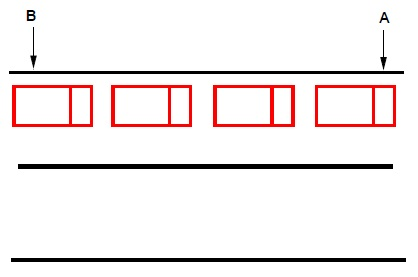
\includegraphics[width=0.7\textwidth]{capitulos/5/figuras/figura1.jpg}
	\caption{\label{fig:densidad} Ilustración de Densidad}	
\end{figure}

\section{Estimación de Tráfico en tiempo real}

Para la estimación de tráfico en tiempo real, los países desarrollados utilizan redes de sensores detectores \cite{leduc2008road} como fuente de datos. Desde el verano de 2007, la Dirección General de Tráfico (DGT) del Ministerio del Interior de España ha estado proveyendo una gran cantidad de datos de tráfico en tiempo real integrados con los mapas de Google. Utilizando unos 4000 sensores de tráfico localizados a lo largo de la red de caminos españoles. Esta herramienta permite, por ejemplo, recolectar el flujo de tráfico por hora y la velocidad promedio en los alrededores de Madrid (\Cref{fig:mapaTrafico}) a través de sensores ubicados en los cruces de las carreteras.

\begin{figure}[h]
	\centering
	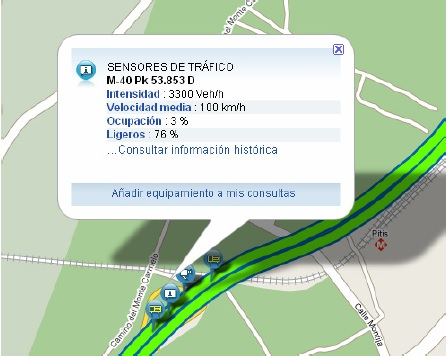
\includegraphics[width=0.7\textwidth]{capitulos/5/figuras/figura2.jpg}
	\caption{\label{fig:mapaTrafico} Típica información proveída por el mapa de tráfico de la DGT}	
\end{figure}

Otros países como Francia, Reino Unido y Portugal cuentan con sistemas similares a los de España. También existen varios estudios basados en FCD para la estimación de tráfico en tiempo real, en \cite{herrera2010evaluation} presentan uno de los primeros experimentos de campo utilizando teléfonos celulares equipados con GPS para obtener datos de tráfico en tiempo real, en el mismo se utilizaron 100 vehículos que llevaban un nokia N95 a bordo. La prueba consistió en conducir en círculos en un tramo de aproximadamente 15 kilómetros de la carretera I-880, cerca de Union City. Los resultados obtenidos del experimento sugerían que una penetración de 2-3\% de teléfonos móviles entre los conductores era suficiente para proveer medidas precisas de la velocidad del flujo de tráfico. En otros trabajos como \cite{reinthaler2007evaluation} se utiliza a taxis como vehículos de prueba para la obtención de FCD, debido a que las medidas de velocidad provenientes de taxis son representativas de la velocidad promedio de toda la población de vehículos \cite{linauer2004fleet}. 

Aparte de la estimación de tráfico, también es posible realizar predicciones del estado del tráfico basándose en la información actual e histórica del tráfico. En \cite{de2008traffic} trabajaron con 600.000 vehículos que enviaban su ubicación cada tres minutos, y a través de dos algoritmos basados en redes neuronales y emparejamiento de patrones realizaban predicciones a corto plazo (15 a 30 minutos) del estado de tráfico futuro. Logrando un error situado entre 2\% a 8\% en predicciones de 15 minutos y 3\% a 16\% para predicciones de 30 minutos.